
\begin{myblock}{Merge-and-Shrink}
\Large
\begin{itemize}
\item Merge-and-Shrink (M\&S) transforms the set of \emph{atomic projections} into a flexible abstraction with three operations: \embl{merge}, \embl{shrink} and \embl{label reduction}.
\end{itemize}

\begin{minipage}{0.3\textwidth}
  \centering
  \raisebox{-0.5\height}{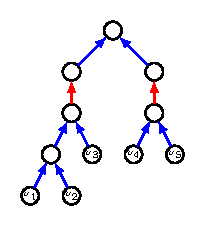
\includegraphics[scale=4]{pdfs/mas/tree.pdf}}
\end{minipage}
\hspace*{1in}
\begin{minipage}{0.5\textwidth}
\begin{algorithm}[H]
\begin{algorithmic}[1]
\STATE $P=\{\text{all atomic projections}\}$
\WHILE{$|P|>=1$}
	\STATE $A_1,A_2=\text{choose-next-merge}(P)$
	\IF{$|A_1|\cdot|A_2|>\text{limit}$}
		\STATE $\text{reduce-labels}(A_1,A_2,S)$
		\STATE $\text{shrink}(A_1,A_2)$
	\ENDIF
\STATE $P=P\cup\{A_1 \otimes A_2\}\setminus\{A_1,A_2\}$
\ENDWHILE
\end{algorithmic}
\caption{Merge-and-Shrink}
\label{alg:seq}
\end{algorithm}

\normalsize
\begin{itemize}
\item which two to merge? $\rightarrow$ merging strategy 
\item how to shrink? $\rightarrow$ shrinking strategy
\item how to reduce labels? $\rightarrow$ label reduction
\end{itemize}
\end{minipage}
\vspace{0.3in}
\begin{itemize}
\item SCC-DFP is the best-performing M\&S in literatures.
\end{itemize}

\end{myblock}

\begin{myblock}{Heuristic Guided Merging Strategy}
\Large
\begin{itemize}
\item The ultimate goal of M\&S is to get a better heuristic.
\item Use \embl{heuristic quality evaluator} to help determine which two abstractions to merge next.
\end{itemize}
\hspace*{1in}
\begin{minipage}{0.8\textwidth}
\begin{itemize}
%\item Evaluate the heuristic quality \embl{improvement} for each pair of abstractions from current pool $S$.
\item \textbf{Q}$_0$ is heuristic on the initial state.
\item \textbf{I}$^+_{\textbf{Q}_0}$ evaluates improvement by comparing \textbf{Q}$_0$ of $A_1 \otimes A_2$ against the sum of \textbf{Q}$_0$ of $A_1$ and $A_2$.
\end{itemize}
\end{minipage}
\vspace*{0.3in}
\begin{itemize}
\item Experiments:
\end{itemize}
\hspace*{0.5in}
\begin{minipage}{0.37\textwidth}
\normalsize
\vspace*{0.3in}
\begin{itemize}
\item IPC benchmarks
\item 39 domains and 1499 tasks
\item 2GB memory / 30 min
\item We compare \embl{coverage} and \embl{number of A* expansions}
\item Results:
\item[\textcolor{blue}{\textbf{+}}] HG solves 36 tasks on which SD fails
\item[\textcolor{red}{\textbf{-}}] but also fails on 26 tasks SD solves
\item[\textcolor{blue}{\textbf{+}}] HG requires fewer expansions than SD in general
\end{itemize}
\end{minipage}
\begin{minipage}{0.57\textwidth}
  \centering
  \raisebox{-0.5\height}{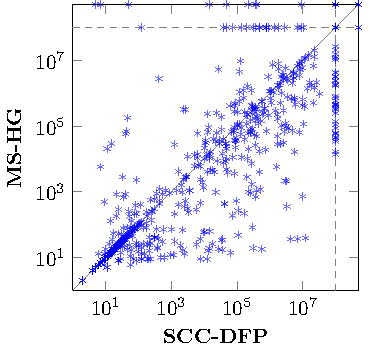
\includegraphics[scale=2.2]{pdfs/figure4.pdf}}
\end{minipage}

\end{myblock}



\begin{myblock}{Issues in Merge-and-Shrink}
\Large
\begin{itemize}
\item M\&S suffers from the expensive construction process:
\end{itemize}

\begin{center}
\begin{minipage}{0.7\textwidth}
\begin{table}
\normalsize 
\centering
\begin{tabular}{|c|c|c|c|c|c|}
\hline\Tstrut
\# Variables & 126 & 169 & 212 & 255 & 298 \\
\hline\Tstrut
 Constr. Time & 157 & 304 & 666 & 1059 & (timeout)\\
\hline
\end{tabular}
\caption{
\normalsize  M\&S construction time (in seconds) on a series of tasks with increasing numbers of variables (atomic projections).}\end{table}
\end{minipage}
\end{center}

\begin{itemize}
\item "passive" shrinking in M\&S is not always the best strategy:
\end{itemize}

\begin{center}
\begin{minipage}{0.7\textwidth}
\begin{table}
\setlength\tabcolsep{5pt}
\centering
\normalsize
\begin{tabular}{|c|c|c|c|c|c|c|}
\hline\Tstrut %\multirow{2}{*}{\hspace{-2pt}\normalsize (b)}
 size limit & MIN & $10^2$ & $10^3$ & $10^4$ & $10^5$ & $10^6$ \\
\hline\Tstrut
 \# expan. & 396 & 9,670 & 21,058 & 44,643 & 14,065 & 9,230 \\
\hline
\end{tabular}
\caption{\normalsize Numbers of nodes expanded by A* using M\&S heuristics constructed with different size limits.}\label{example:2}
\end{table}
\end{minipage}
\end{center}


\end{myblock}

